\section{Model Validation with Simulated Scenarios}
\label{sec:model-validation}

The validation of the proposed model was conducted using a close-to-realistic scenario based on the building layout presented in \cite{ref-mdpi-2025}, as illustrated in Figure~\ref{fig:building-layout}.

\begin{figure}[ht]
\centering
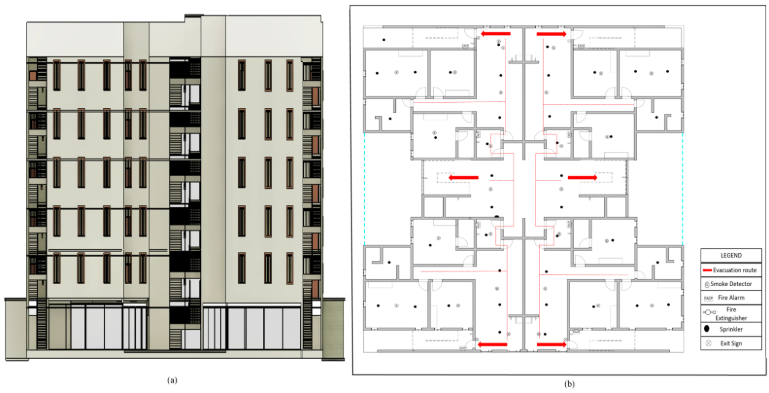
\includegraphics[width=0.85\textwidth]{figures/building.png}
\caption{Building layout used for the simulation scenario.}
\label{fig:building-layout}
\end{figure}

Due to practical limitations and the infeasibility of implementing and testing the system in a real-world fire emergency environment, a simulation environment was developed to emulate the behavior of the building during a fire incident.

The floor layout is divided into cells according to the building structure, including the locations of rooms, corridors, walls, and alarms. Each cell represents a spatial unit where fire spread, smoke propagation, and rescue operations may occur. The cells are indexed sequentially starting from the top-left corner of the grid, with indices ranging from 0 to $6 \times 7 - 1 = 41$. The resulting indexing scheme is shown in Figure~\ref{fig:index-matrix}.

\begin{figure}[ht]
\centering
\includegraphics[width=0.7\textwidth]{figure-B-index-matrix} % replace with actual filename
\caption{Index matrix of the $6 \times 7$ grid (0 to 41).}
\label{fig:index-matrix}
\end{figure}

The simulation time is divided into discrete time periods, representing the progression of the fire incident. Each period corresponds to a fixed time interval after the initial ignition. In the visualization matrices, these time intervals are denoted as $t = 0, 1, 2, 3,$ and $4$. It is assumed that both fire and smoke propagation rates remain constant throughout the simulation, meaning that the cell size does not change across periods. Consequently, the predicted fire arrival times, smoke arrival times, and population distributions remain fixed for each cell during the simulation.

Population distribution varies across the building layout, reflecting typical human occupancy patterns. In particular, population density is slightly higher in rooms where most people tend to congregate, compared to other spaces such as corridors and transitional areas, which contain fewer people.

To initialize the scenario, five matrices are defined to represent the environmental and operational conditions of the building. These matrices describe the fire arrival time, smoke arrival time, population distribution, asset value, and minimum suppression rate required for each cell. The matrices are presented in Figure~\ref{fig:input-matrices} (a)--(e). According to the fire arrival time matrix, the fire ignites from the cell with a value equal to 0 and subsequently spreads to neighboring cells over time.

\begin{figure}[ht]
\centering
\begin{subfigure}{0.32\textwidth}
    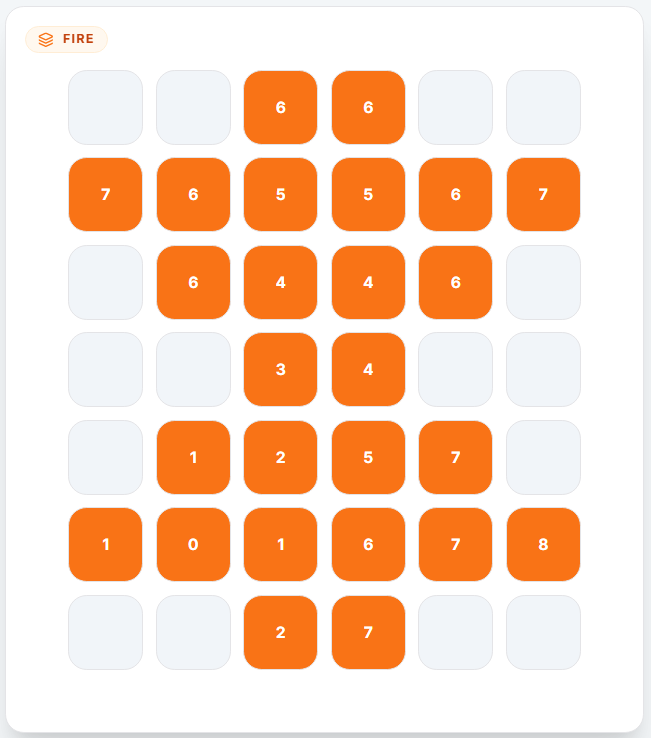
\includegraphics[width=\textwidth]{figures/3fire.png} % placeholder
    \caption{Fire arrival time matrix}
    \label{fig:fire-arrival}
\end{subfigure}
\hfill
\begin{subfigure}{0.32\textwidth}
    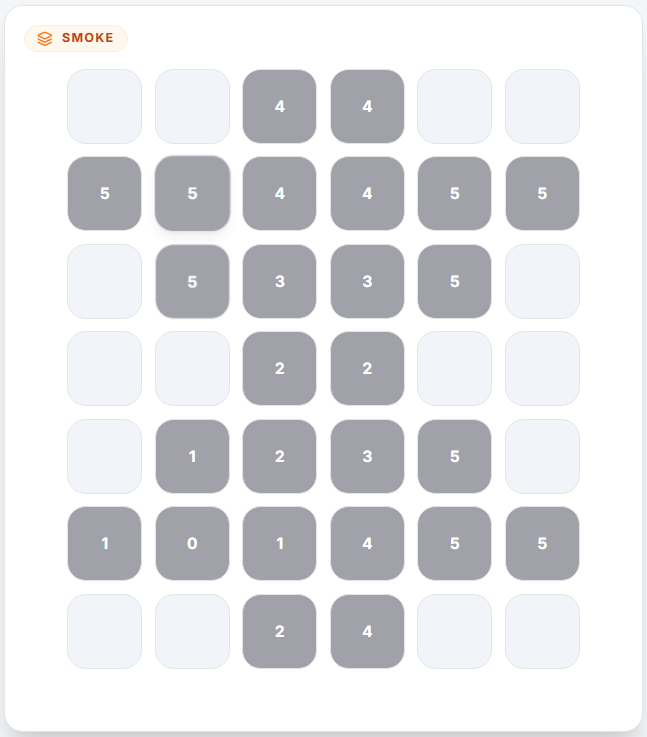
\includegraphics[width=\textwidth]{figures/3smoke.png}
    \caption{Smoke arrival time matrix}
    \label{fig:smoke-arrival}
\end{subfigure}
\hfill
\begin{subfigure}{0.32\textwidth}
    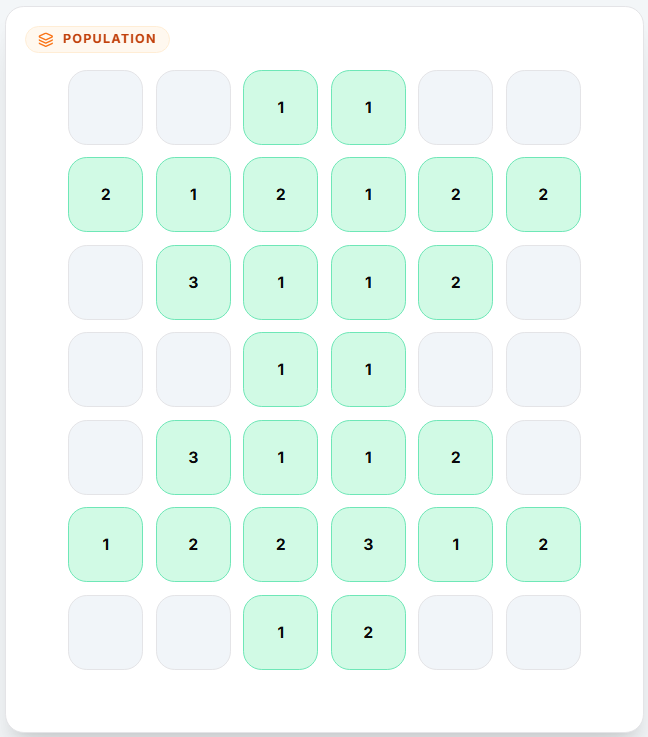
\includegraphics[width=\textwidth]{figures/3population.png}
    \caption{Population distribution matrix}
    \label{fig:population}
\end{subfigure}

\vspace{1em}

\begin{subfigure}{0.32\textwidth}
    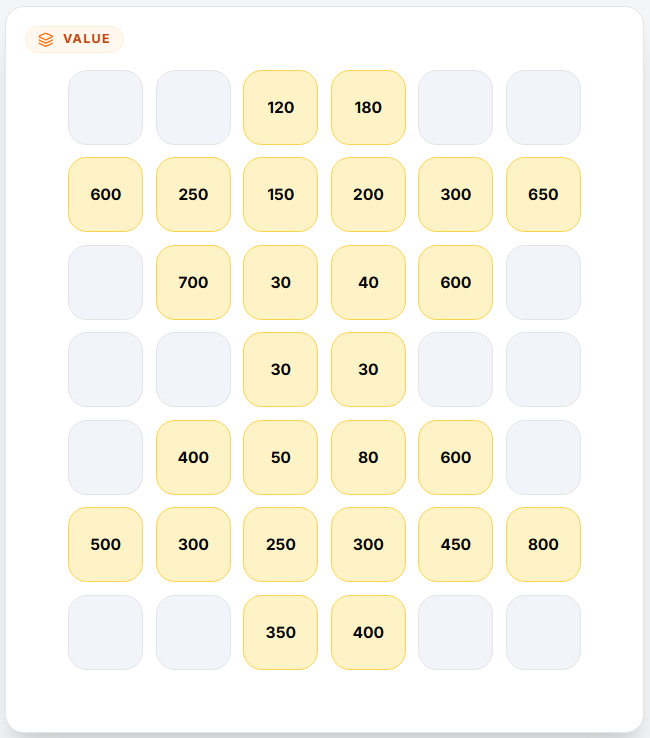
\includegraphics[width=\textwidth]{figures/3value.png}
    \caption{Asset value matrix}
    \label{fig:value}
\end{subfigure}
\hfill
\begin{subfigure}{0.32\textwidth}
    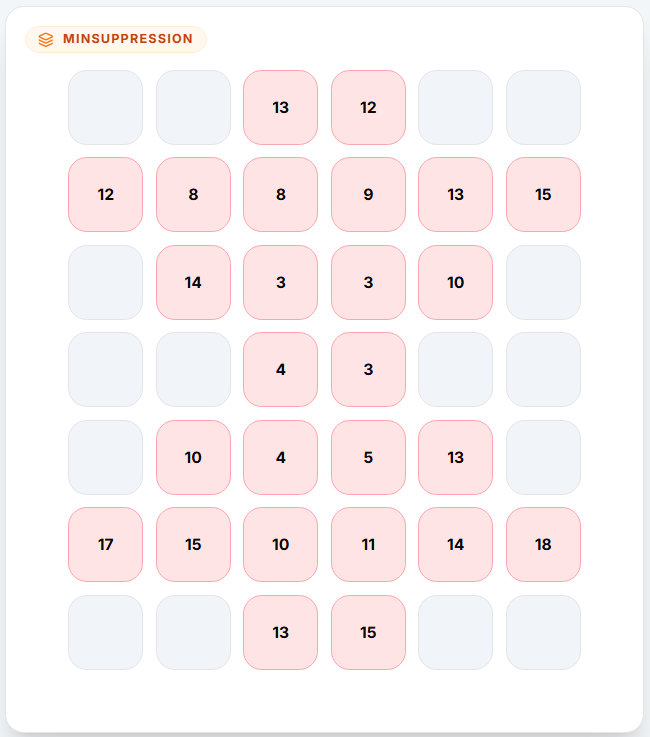
\includegraphics[width=\textwidth]{figures/3min.png}
    \caption{Minimum suppression rate matrix}
    \label{fig:minsuppression}
\end{subfigure}

\caption{Input matrices for the simulation: (a) FIRE, (b) SMOKE, (c) POPULATION, (d) VALUE, (e) MINSUPPRESSION.}
\label{fig:input-matrices}
\end{figure}

In this validation scenario, it is assumed that there are six different resource types of response teams: three suppression-oriented teams and three rescue-oriented teams. Each resource type is characterized by its suppression capability, rescue capability, deployment cost, and availability over time. The parameters of these resource teams are given in Table~\ref{tab:resource-teams}. The total operational budget available for resource deployment is set to 500.

\begin{table}[ht]
\centering
\caption{Resource Teams and Their Capacities Over Time}
\label{tab:resource-teams}
\begin{tabular}{c c c l}
\hline
\textbf{Resource Type} & \textbf{Suppression Rate} & \textbf{Cost} & \textbf{Capacity (Availability by Time Slot)} \\ 
\hline
A & 3 & 8 & 
\begin{tabular}[t]{@{}l@{}}
$t=0$:1 \\ 
$t=1$:2 \\ 
$t=2$:1 \\ 
$t=3$:2 \\ 
$t=4$:2 
\end{tabular} \\ 
B & 5 & 18 & 
\begin{tabular}[t]{@{}l@{}}
$t=0$:1 \\ 
$t=1$:2 \\ 
$t=2$:0 \\ 
$t=3$:1 \\ 
$t=4$:2 
\end{tabular} \\ 
C & 7 & 35 & 
\begin{tabular}[t]{@{}l@{}}
$t=0$:0 \\ 
$t=1$:2 \\ 
$t=2$:0 \\ 
$t=3$:1 \\ 
$t=4$:2 
\end{tabular} \\ 
D & 0 & 7 & 
\begin{tabular}[t]{@{}l@{}}
$t=0$:1 \\ 
$t=1$:2 \\ 
$t=2$:1 \\ 
$t=3$:1 \\ 
$t=4$:3 
\end{tabular} \\ 
E & 0 & 16 & 
\begin{tabular}[t]{@{}l@{}}
$t=0$:0 \\ 
$t=1$:1 \\ 
$t=2$:2 \\ 
$t=3$:2 \\ 
$t=4$:1 
\end{tabular} \\ 
F & 1 & 37 & 
\begin{tabular}[t]{@{}l@{}}
$t=0$:0 \\ 
$t=1$:1 \\ 
$t=2$:0 \\ 
$t=3$:1 \\ 
$t=4$:2 
\end{tabular} \\ 
\hline
\end{tabular}
\end{table}

The accessibility constraint is defined such that all response operations can only be performed by ground crews. Consequently, all six resource types are considered ground-based units and can only access cells that are reachable through the building’s floor layout. In the accessibility matrix, cells that can be accessed by ground crews are marked with a value of 0. In contrast, inaccessible areas (including structural barriers, non-operational spaces, areas with no population, or locations without alarm coverage) are represented by a value of -1.

During each simulation period, the optimization framework determines how available response teams should be allocated across the grid cells. The objective is to minimize the number of vulnerable individuals exposed to fire and smoke hazards while simultaneously reducing property loss and maintaining deployment costs within the available budget.

The optimal deployment strategies given by the model over the simulation time for this constrained optimization problem are illustrated in Figures~\ref{fig:t0}--\ref{fig:t4}.

\begin{figure}[ht]
\centering
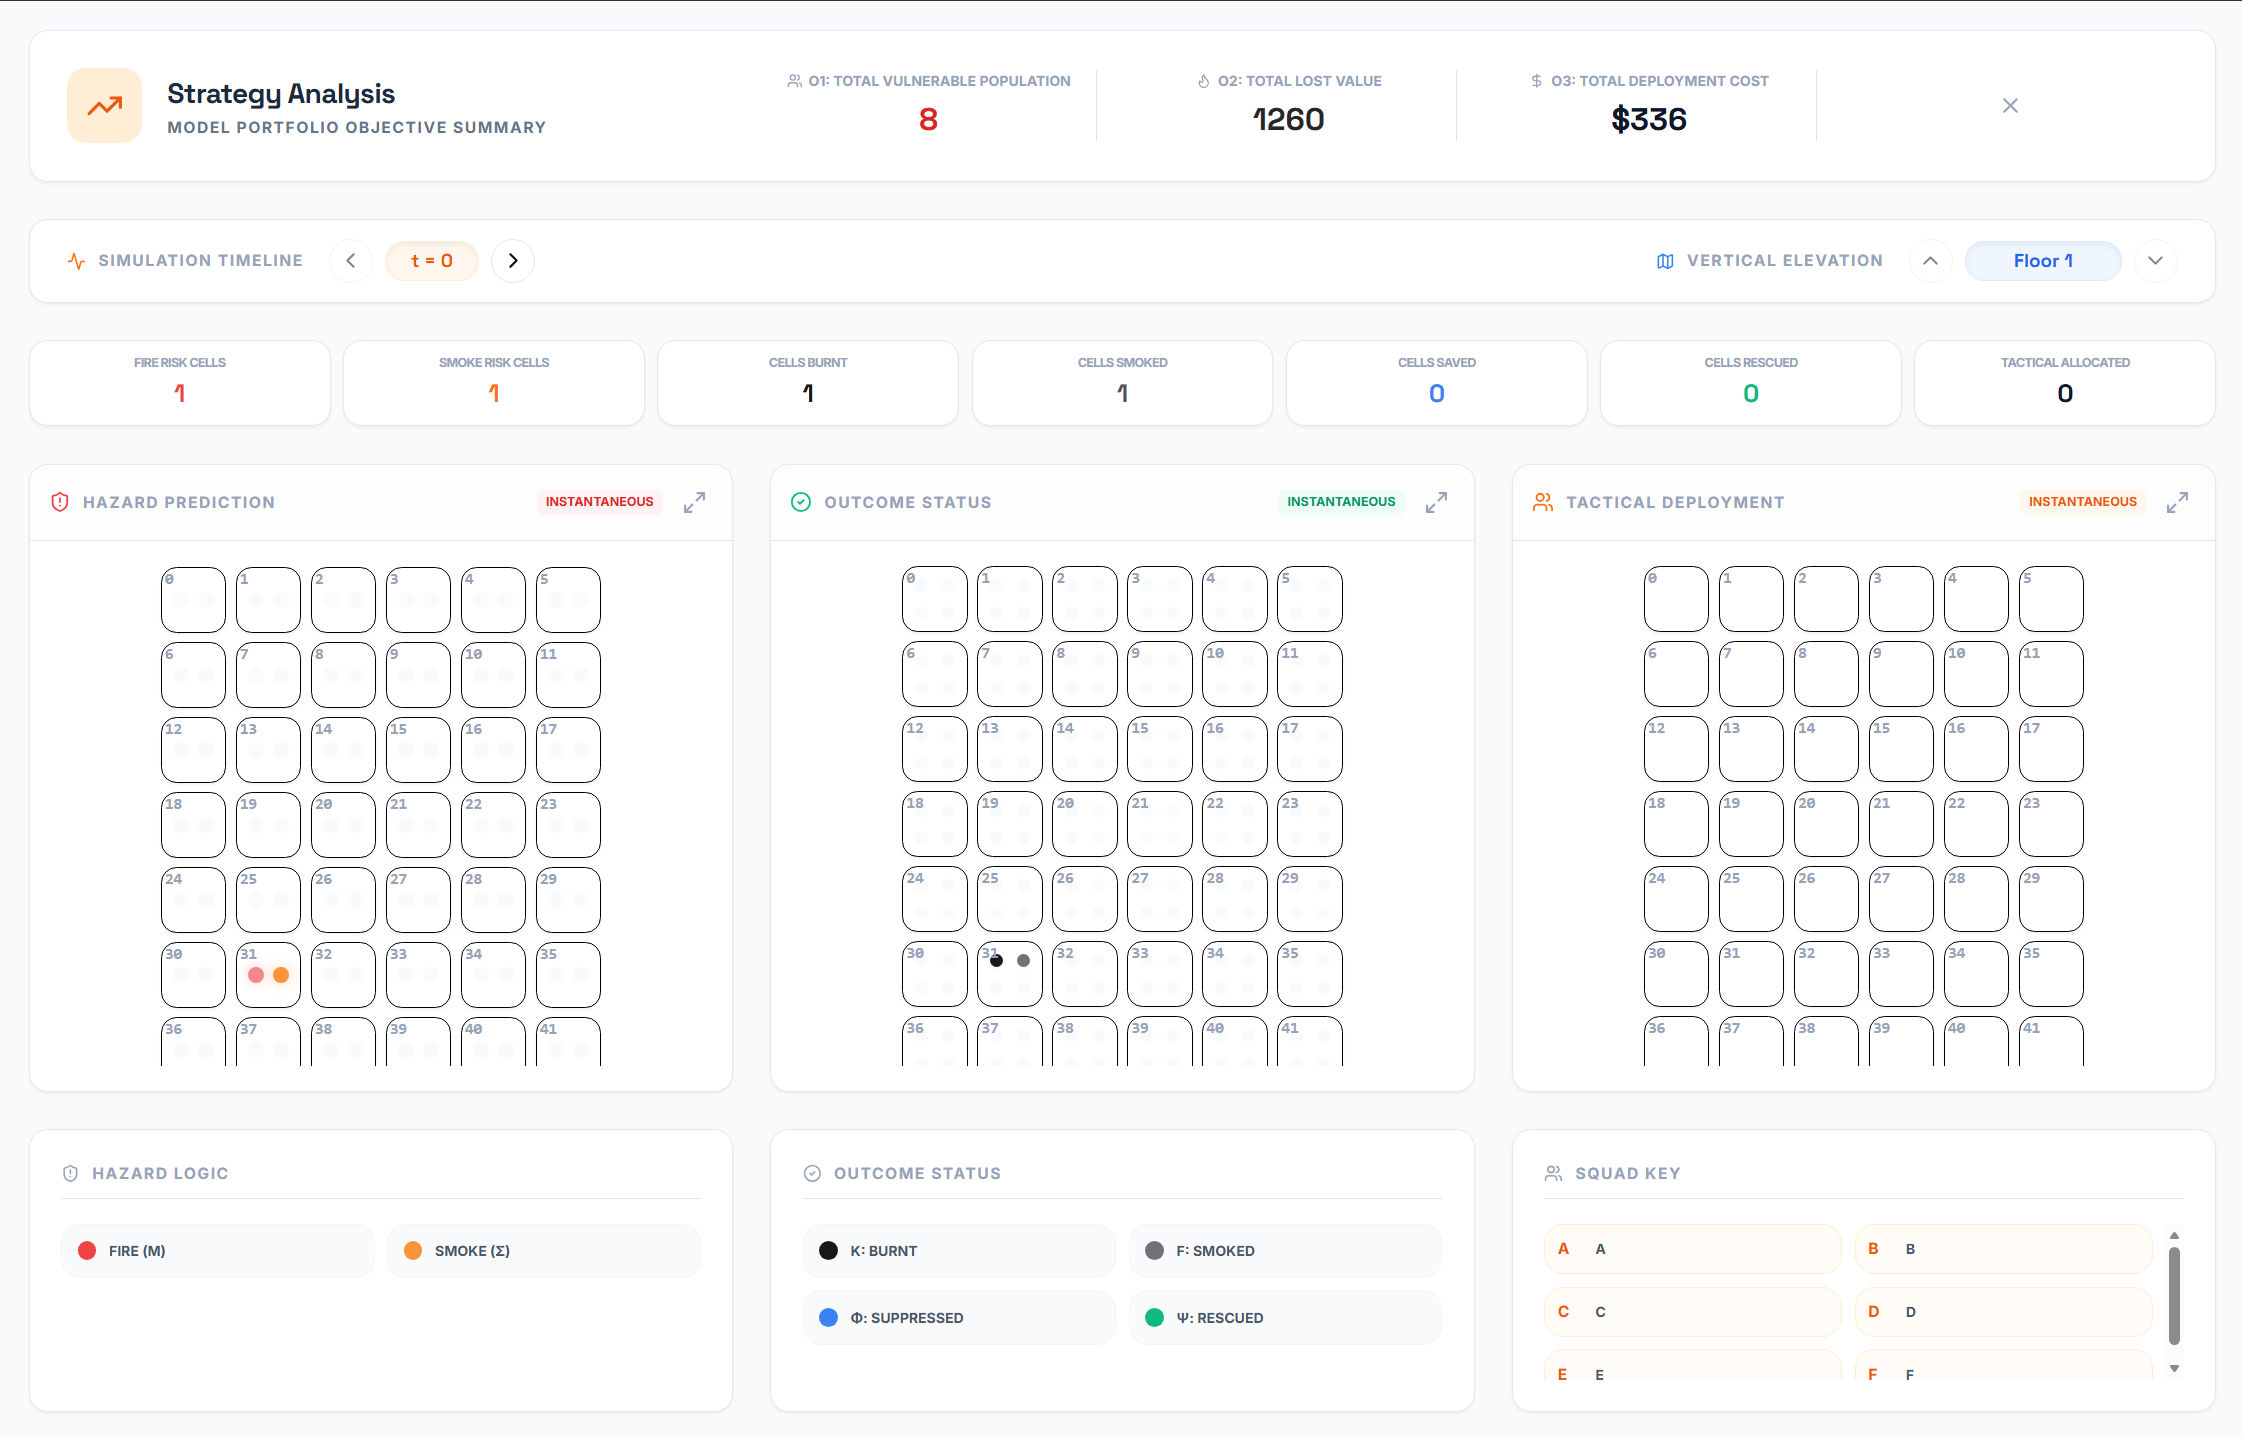
\includegraphics[width=0.9\textwidth]{figures/3t0.png} % placeholder
\caption{Simulation results at $t=0$.}
\label{fig:t0}
\end{figure}

\begin{figure}[ht]
\centering
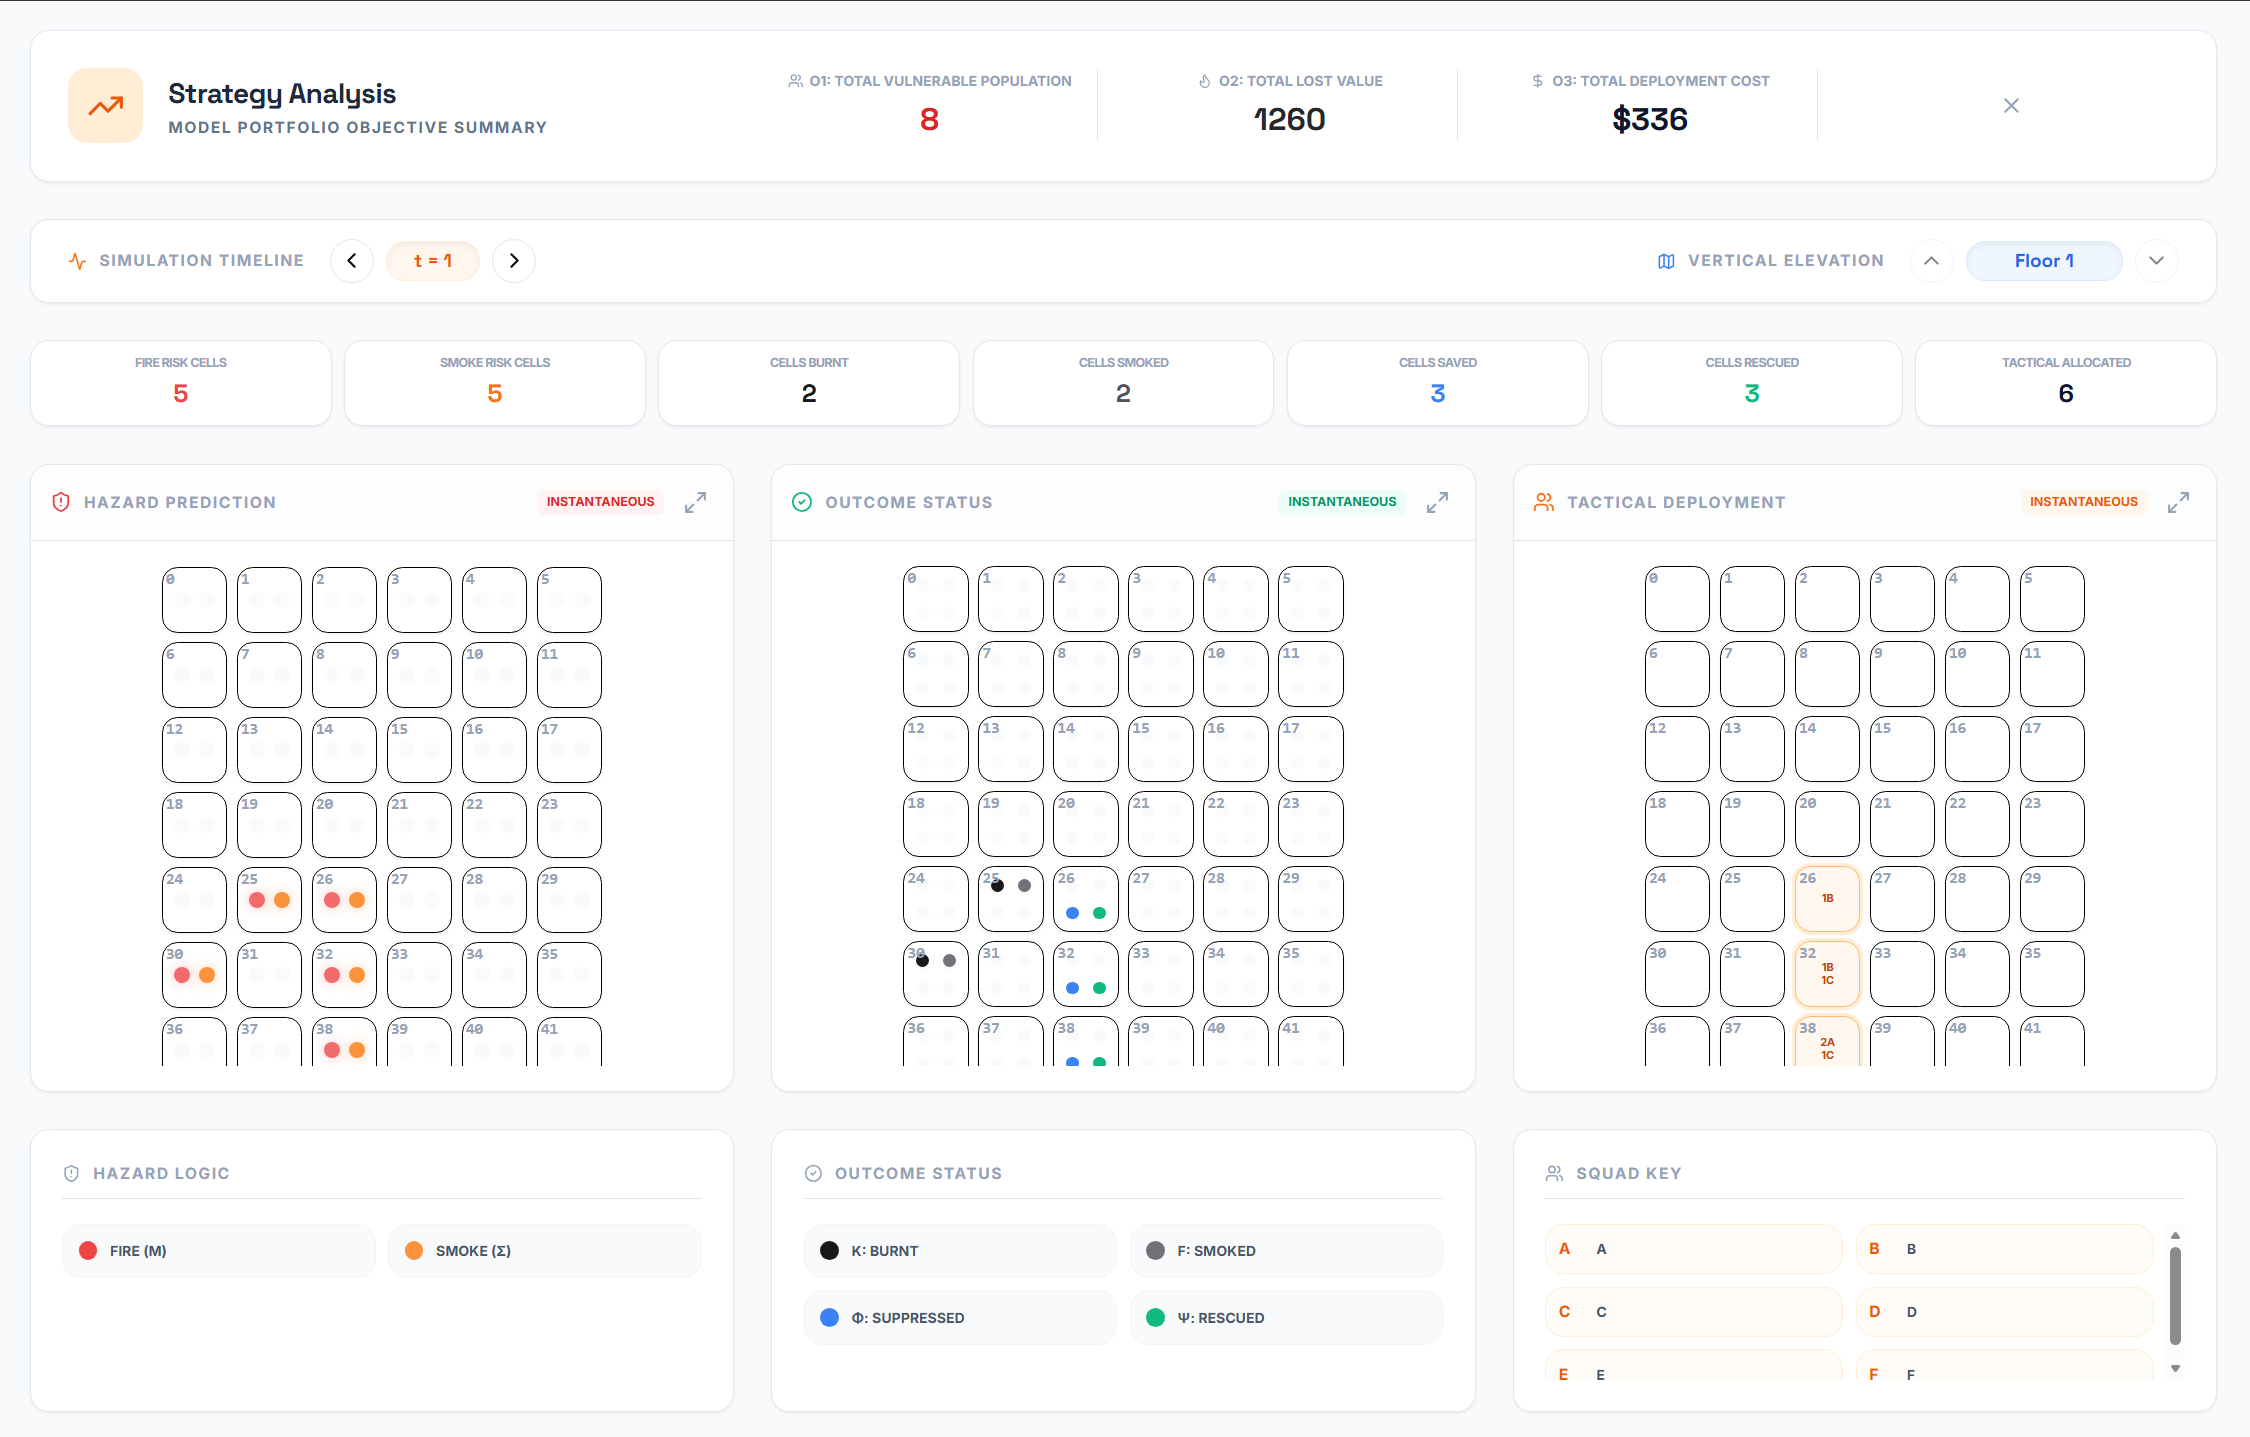
\includegraphics[width=0.9\textwidth]{figures/3t1.png} % placeholder
\caption{Simulation results at $t=1$.}
\label{fig:t1}
\end{figure}

\begin{figure}[ht]
\centering
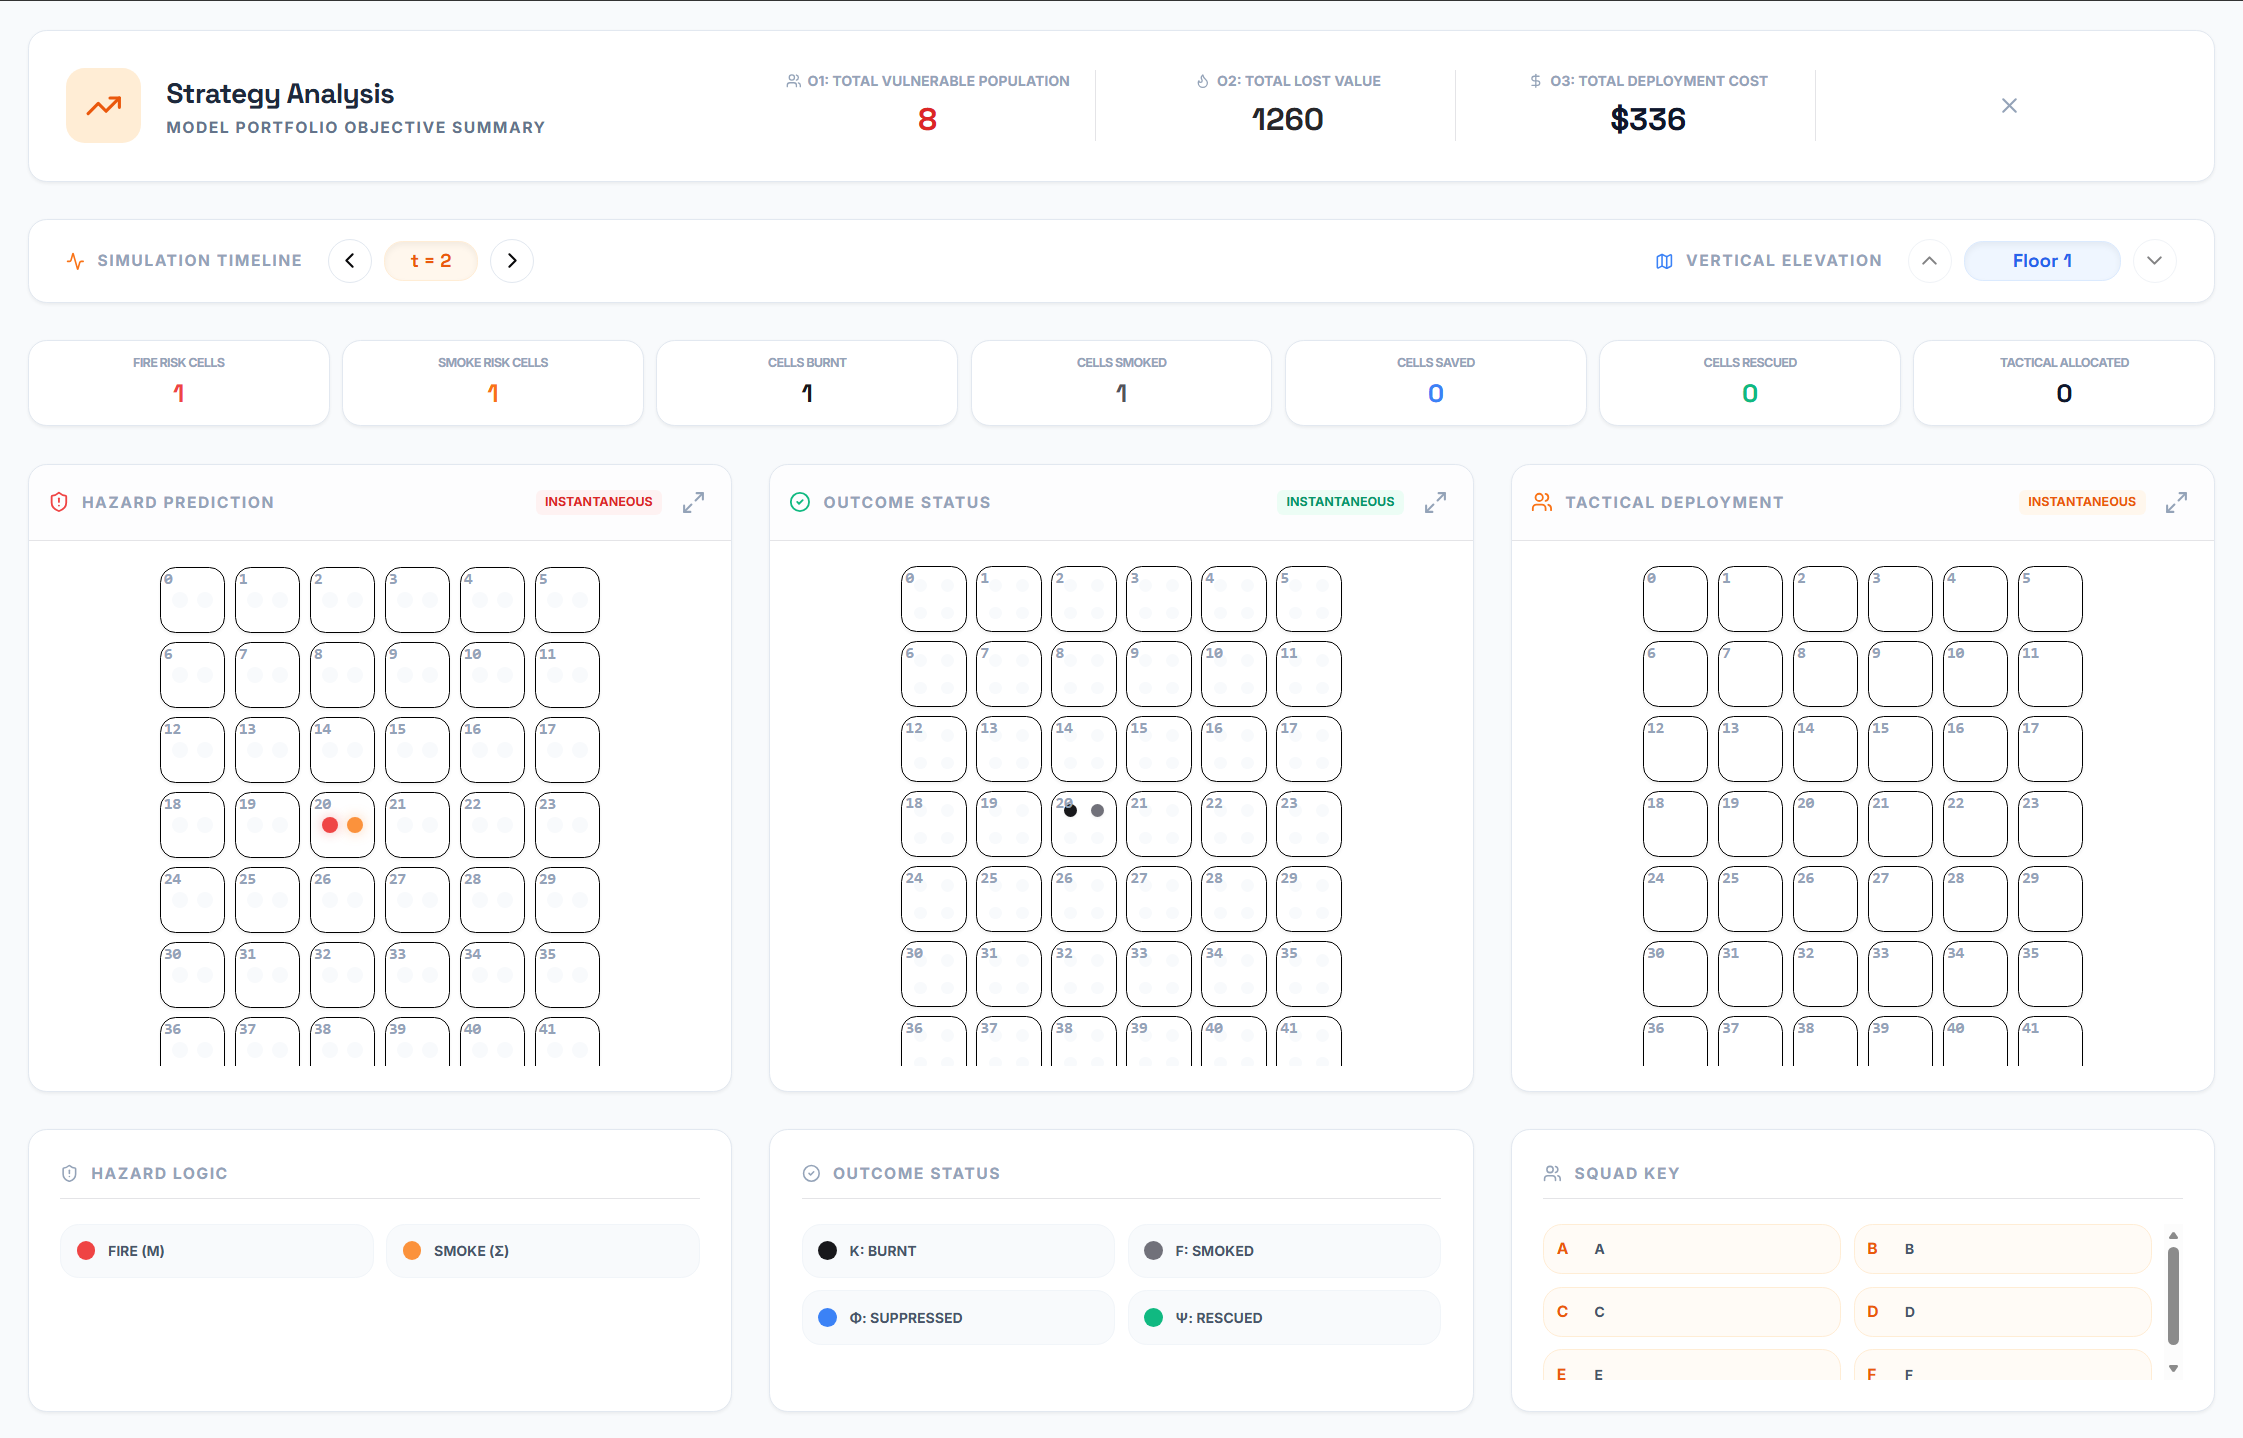
\includegraphics[width=0.9\textwidth]{figures/3t2.png} % placeholder
\caption{Simulation results at $t=2$.}
\label{fig:t2}
\end{figure}


\begin{figure}[ht]
\centering
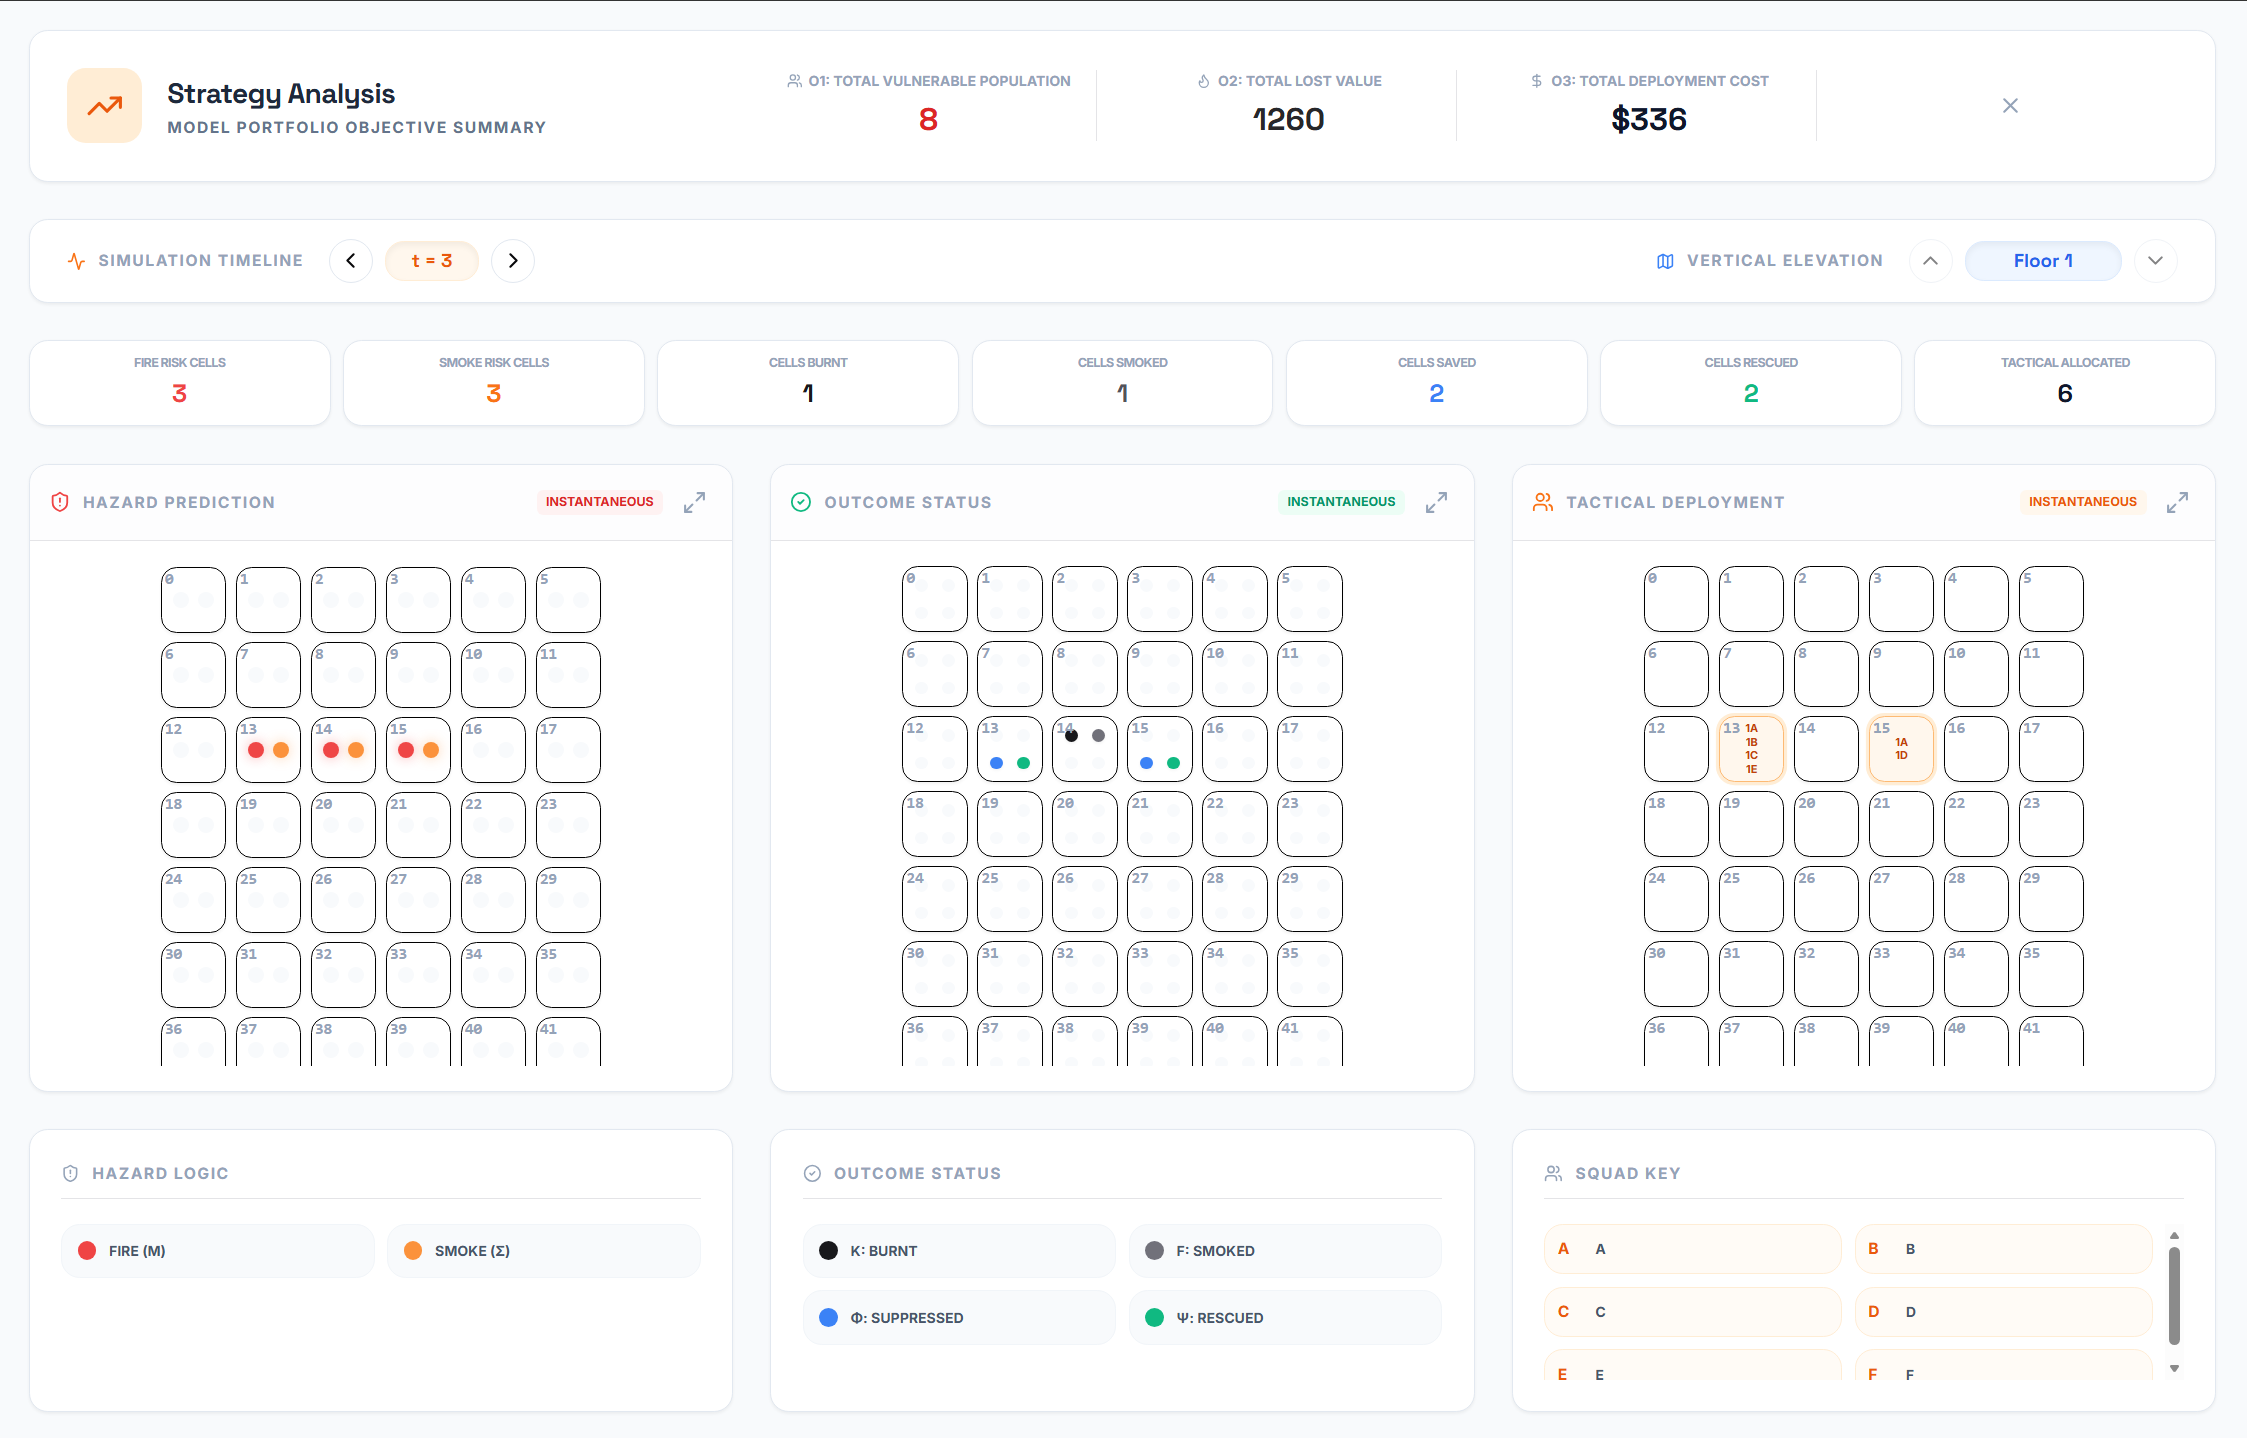
\includegraphics[width=0.9\textwidth]{figures/3t3.png} % placeholder
\caption{Simulation results at $t=3$.}
\label{fig:t3}
\end{figure}

\begin{figure}[ht]
\centering
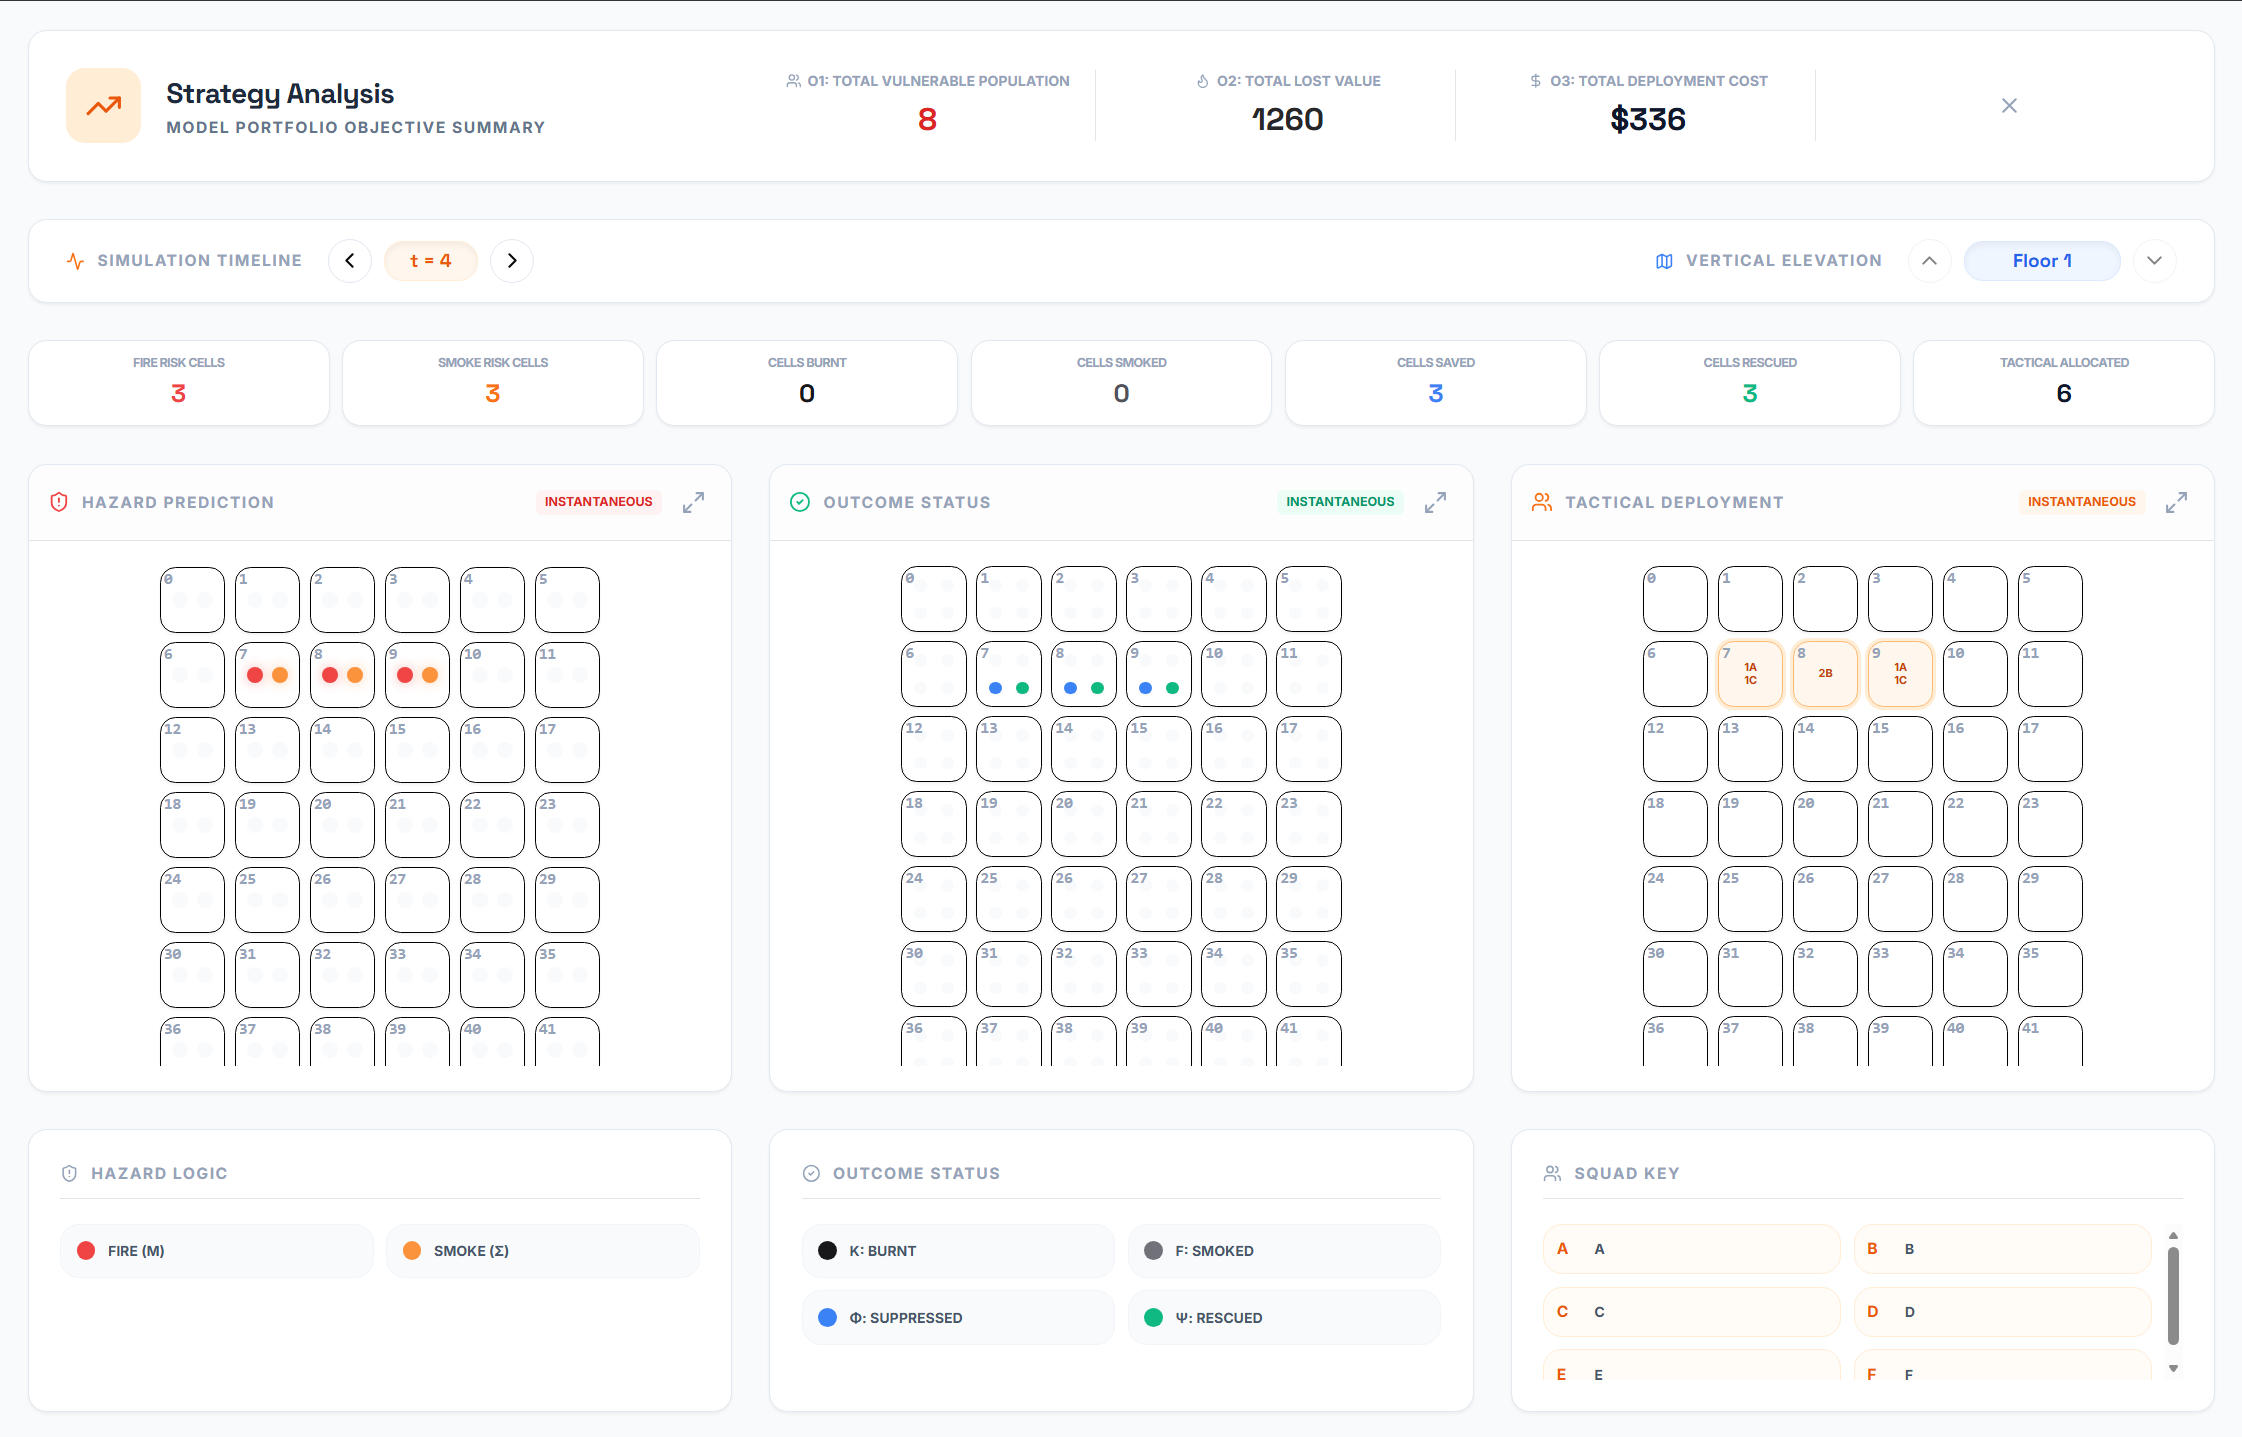
\includegraphics[width=0.9\textwidth]{figures/3t4.png} % placeholder
\caption{Simulation results at $t=4$.}
\label{fig:t4}
\end{figure}

At $t=0$, the system detects the initial ignition point and evaluates the potential fire and smoke spread across the grid. … [continue describing each time step as in your original text]

In summary, the model provides recommendations for allocating the available resources of response teams across specific cells, with the objective of reducing both the total population at risk and the total cells burnt, while still maintaining a reasonable total cost of operation. It also prevents the fire from spreading to the rest of the floor, helping to further minimize damage to property and people.